\RequirePackage{amsmath}
\documentclass[twocolumn, times]{aastex631}
\usepackage[spanish,es-minimal,english]{babel}
\usepackage[utf8]{inputenc}
\usepackage{natbib}
%\usepackage{microtype}
\usepackage{hyperref}
\usepackage{savesym}
\savesymbol{tablenum}
\usepackage{siunitx}
\restoresymbol{SIX}{tablenum}
\usepackage[varg]{newtxmath}
\usepackage{newtxtext}
\usepackage{booktabs}
\usepackage{array}   % for \newcolumntype macro
\newcolumntype{L}{>{$}l<{$}} % math-mode version of lrc column types
\newcolumntype{R}{>{$}r<{$}} 
\newcolumntype{C}{>{$}c<{$}} 

\bibliographystyle{aasjournal}

\newcommand\ION[2]{#1\,\scalebox{0.9}[0.8]{\uppercase{#2}}}
\newcounter{ionstage}
\renewcommand{\ion}[2]{\setcounter{ionstage}{#2}% 
  \ensuremath{\mathrm{#1\,\scriptstyle\Roman{ionstage}}}}
\newcommand\hii{\ion{H}{2}}
\newcommand\sii{[\ion{S}{2}]}
\newcommand\oiii{[\ion{O}{3}]}
\newcommand\Raman{\ensuremath{_{\text{Raman}}}}
\def\th#1#2{\(\theta^{#1}\)\,Ori~#2}
\newcommand\wn{\ensuremath{\tilde{\nu}}}

% Chemical formulae
\newcommand*\chem[1]{\ensuremath{\mathrm{#1}}}
% Atomic term symbols
\newcommand\Config[1]{\ensuremath{\mathrm{#1}}}
\newcommand\Term[3]{\ensuremath{\mathrm{#1\ ^{#2}#3}}}
\newcommand\Level[4]{\ensuremath{\mathrm{#1\ ^{#2}#3_{#4}}}}

\newcommand\ha{\ensuremath{\text{H}\alpha}}
\newcommand\lya{\ensuremath{\text{Ly}\alpha}}
\newcommand\lyb{\ensuremath{\text{Ly}\beta}}

\begin{document}
\title{Raman scattering in a massive young star in the Small Magellanic Cloud}
\shorttitle{Extinction anomalies in the Orion Nebula}
\author{William J. Henney}
\affiliation{%
  \foreignlanguage{spanish}{Instituto de Radioastronomía y
    Astrofísica, Universidad Nacional Autónoma de México, Apartado
    Postal 3-72, 58090 Morelia, Michaoacán, Mexico}}
\email{w.henney@irya.unam.mx}

\begin{abstract}
  I present the first detection of Raman-scattered wings to the \ha{} line in a massive young stellar object (mYSO)
\end{abstract}

\keywords{Atomic physics; Radiative transfer; Photodissociation regions}

%\object{M42}

\section{Introduction}
\label{sec:introduction}




\section{Observations}
\label{sec:observations}




\begin{figure}
  \centering
  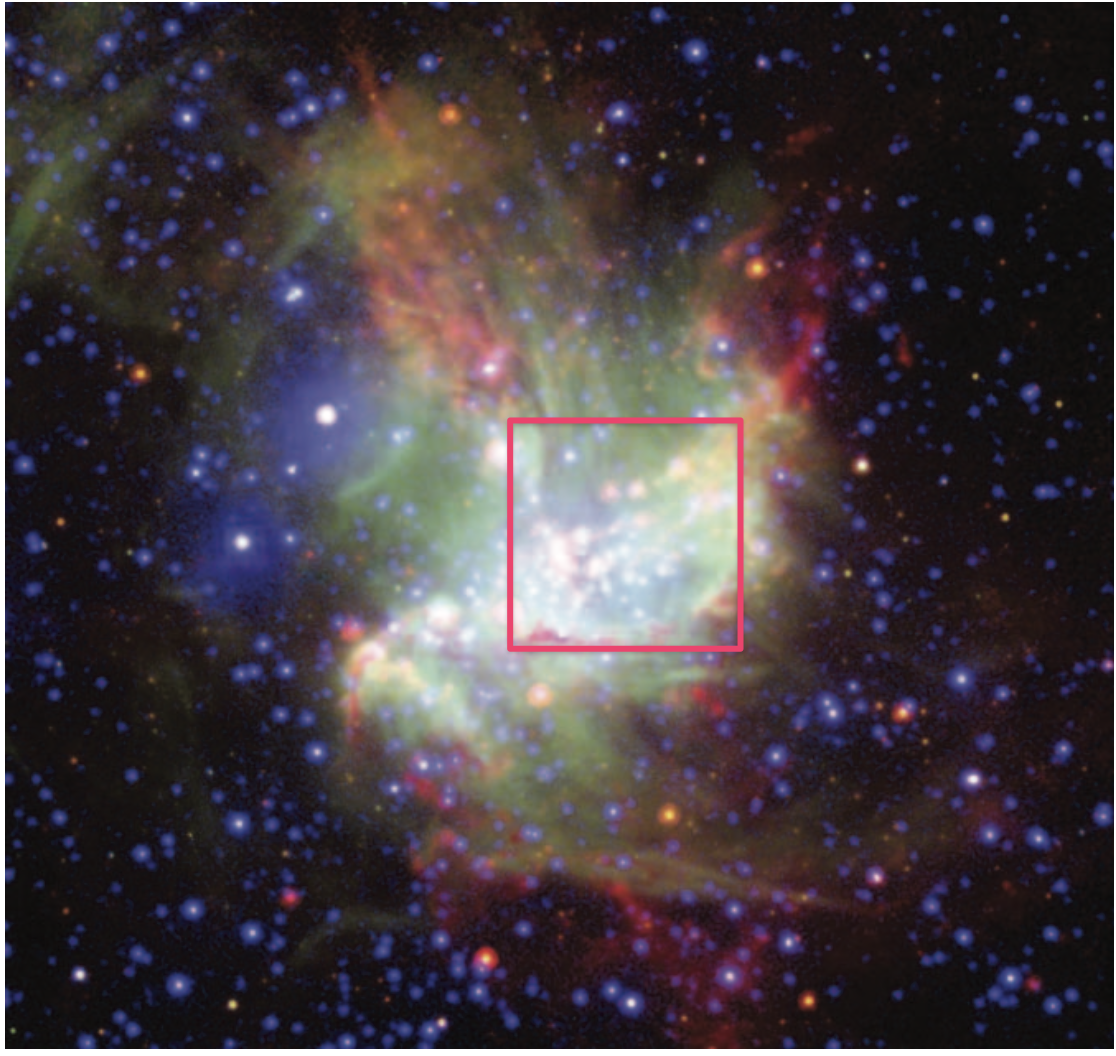
\includegraphics[width=\linewidth]{figs/CleanShot-2021-05-19-gouliermis-fig01}
  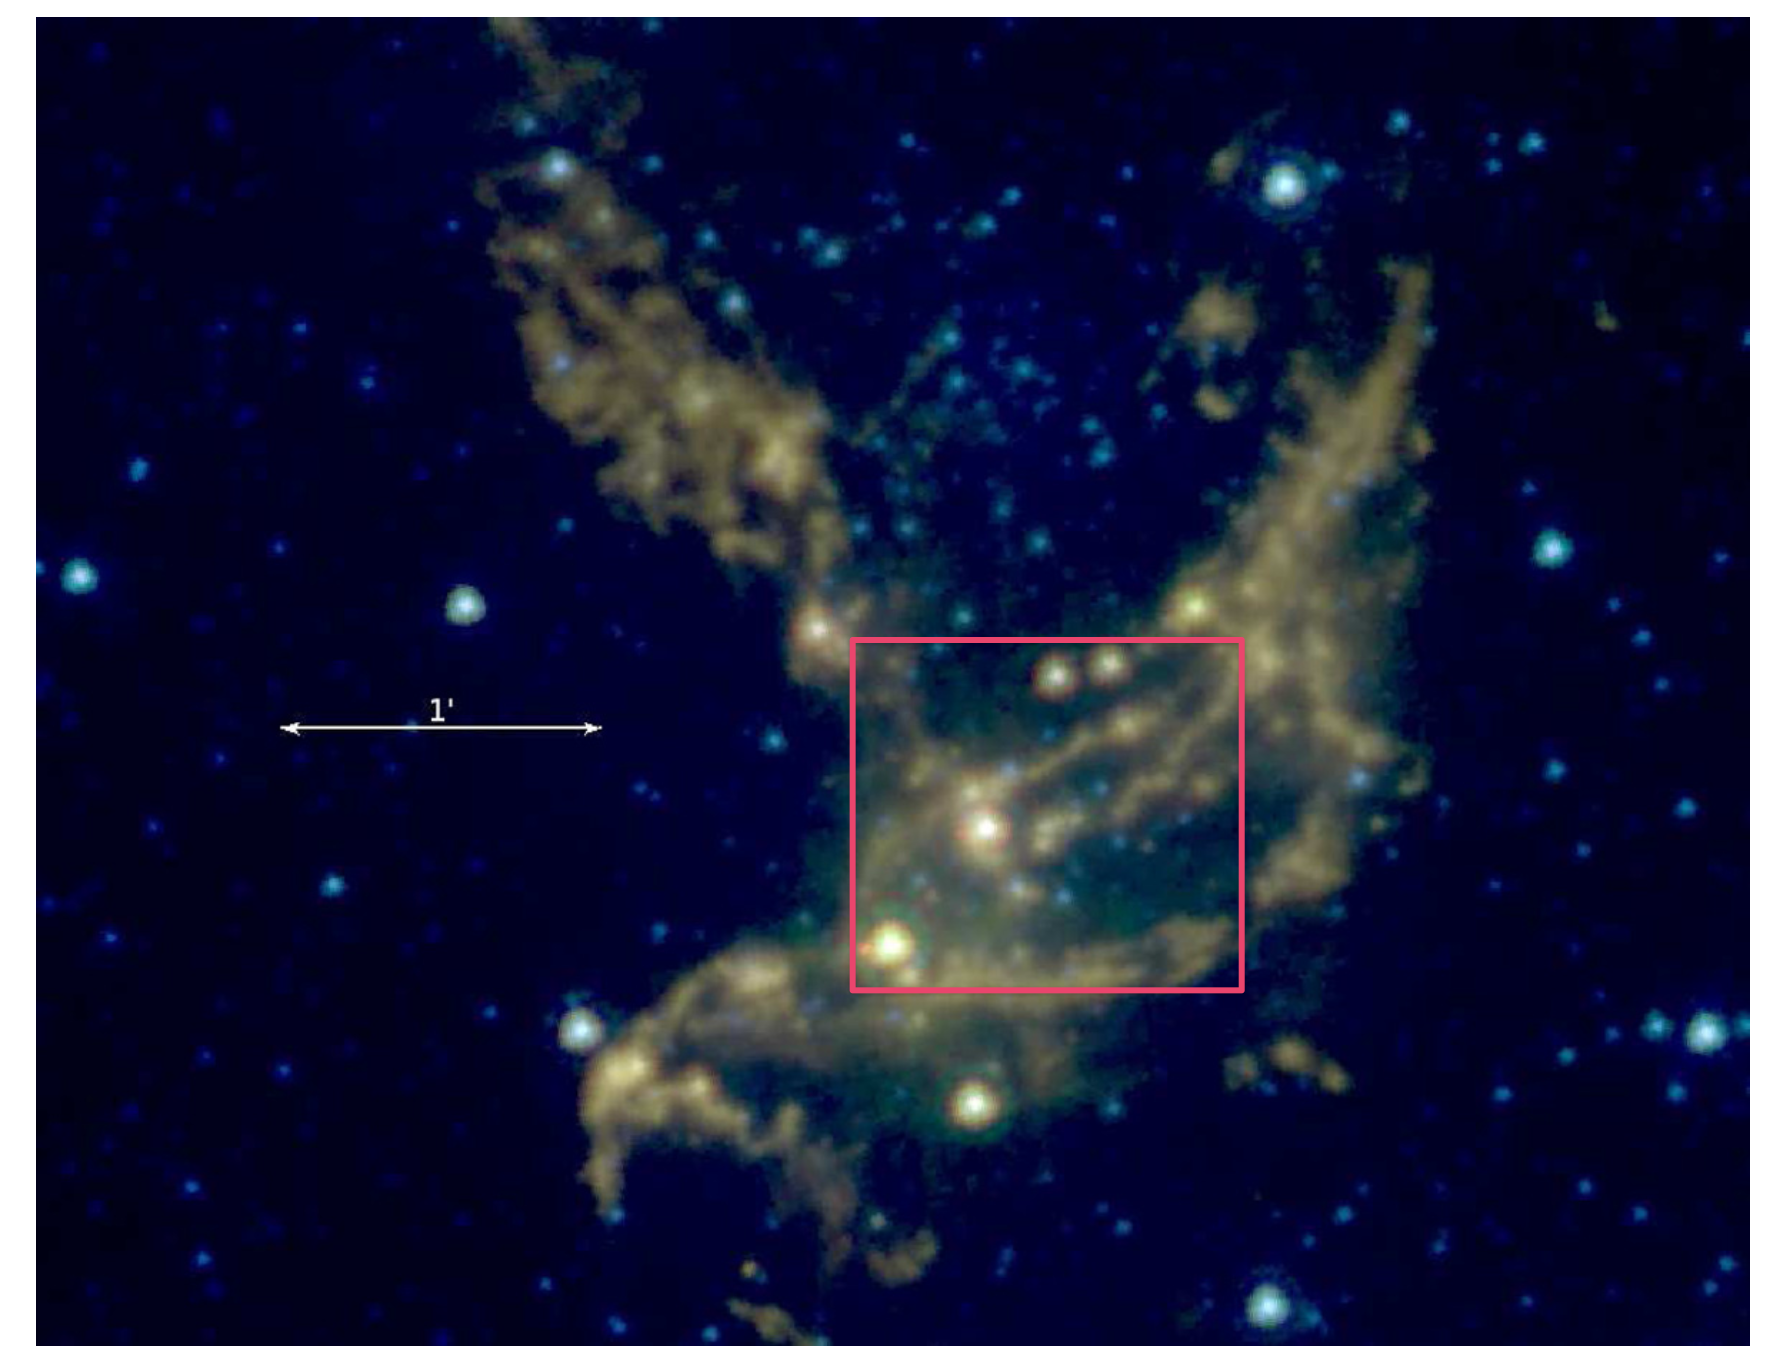
\includegraphics[width=\linewidth]{figs/CleanShot-2021-05-19-whelan-fig01}
  \caption{MUSE field of view (red box)
    shown superimposed on (a) a composite optical/X-ray image of the N~66/NGC~346 region
    from \citet{Gouliermis:2008a} and (b) a Spitzer mid-infrared image \citep{Whelan:2013d}.
  }
  \label{fig:muse-fov}
\end{figure}

\section{Results}
\label{sec:results}

\begin{figure}
  \centering
  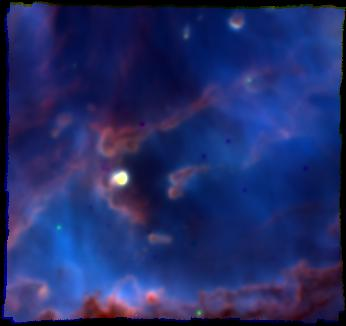
\includegraphics[width=0.8\linewidth]{figs/ngc346-rgb}
  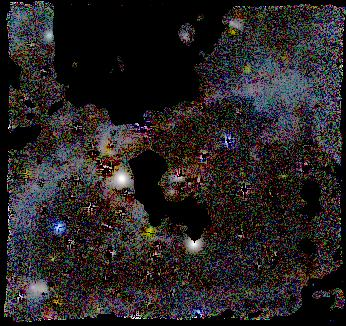
\includegraphics[width=0.8\linewidth]{figs/ngc346-rgb-raman}
  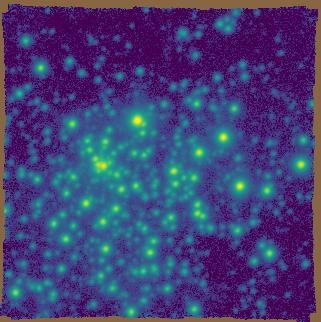
\includegraphics[width=0.8\linewidth]{figs/ngc346-stars}
  \caption{
    (a) Color composite emission line map: \sii{}, \ha{}, \oiii.
    (b) Color composite Raman wing map
    (c) Continuum map.
  }
  \label{fig:random-results}
\end{figure}

\begin{figure*}
  \centering
  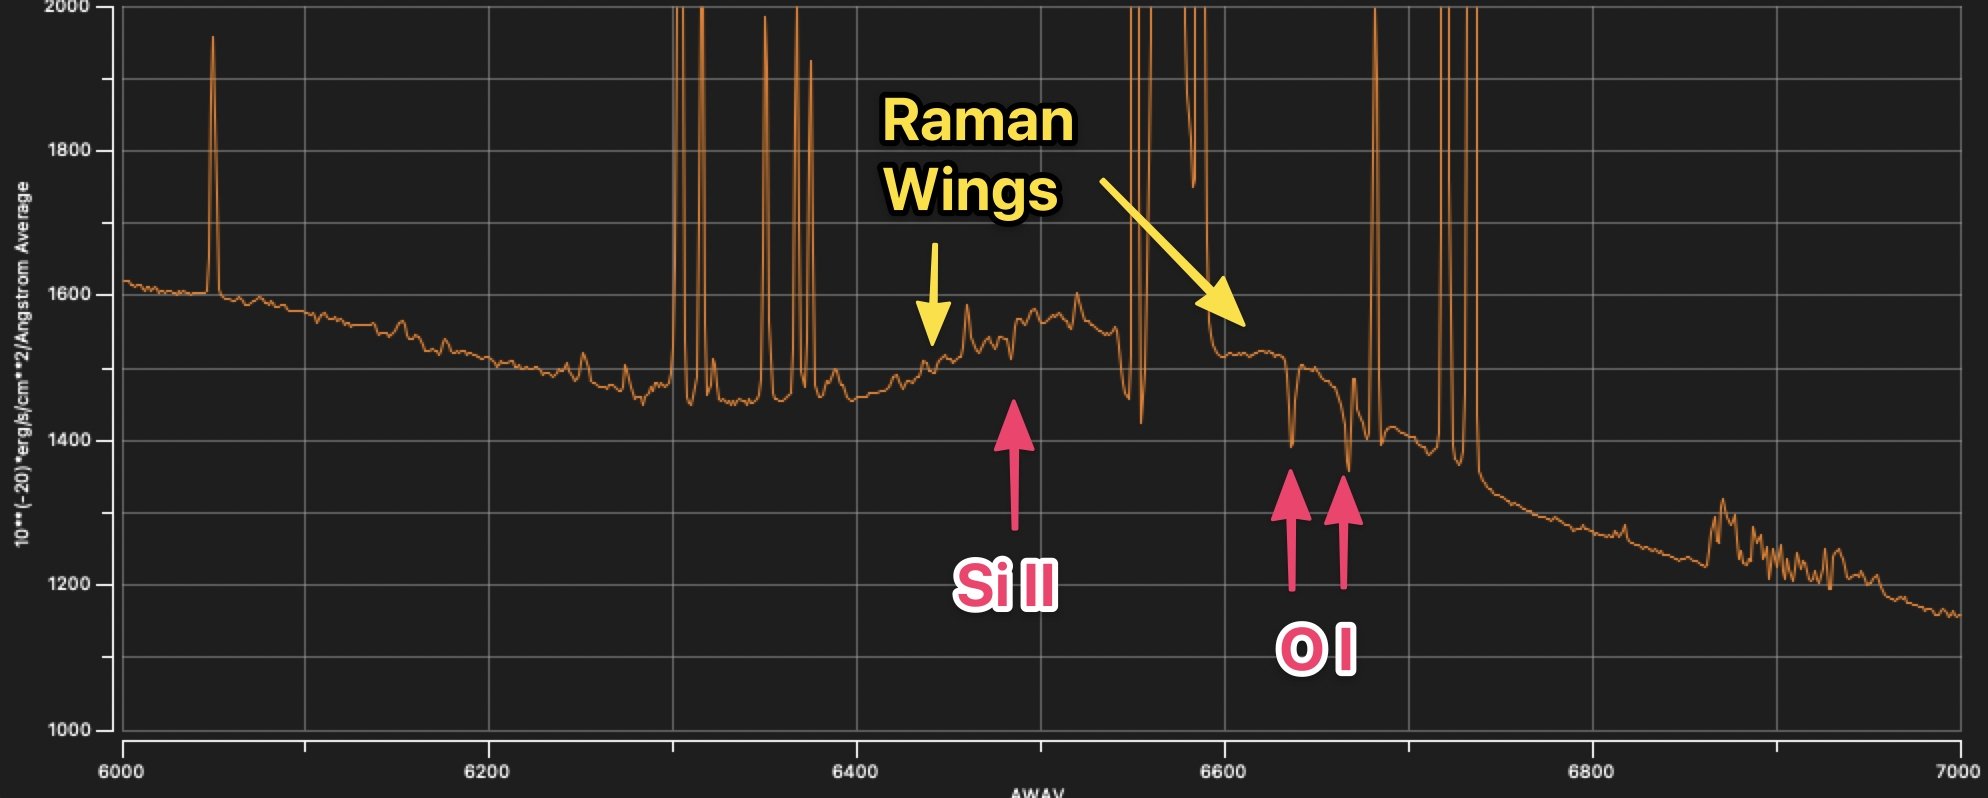
\includegraphics[width=\linewidth]{figs/CleanShot-2021-05-19-Raman-spectrum}
  \caption{The actual spectrum}
  \label{fig:spectrum}
\end{figure*}

\begin{figure*}
  \centering
  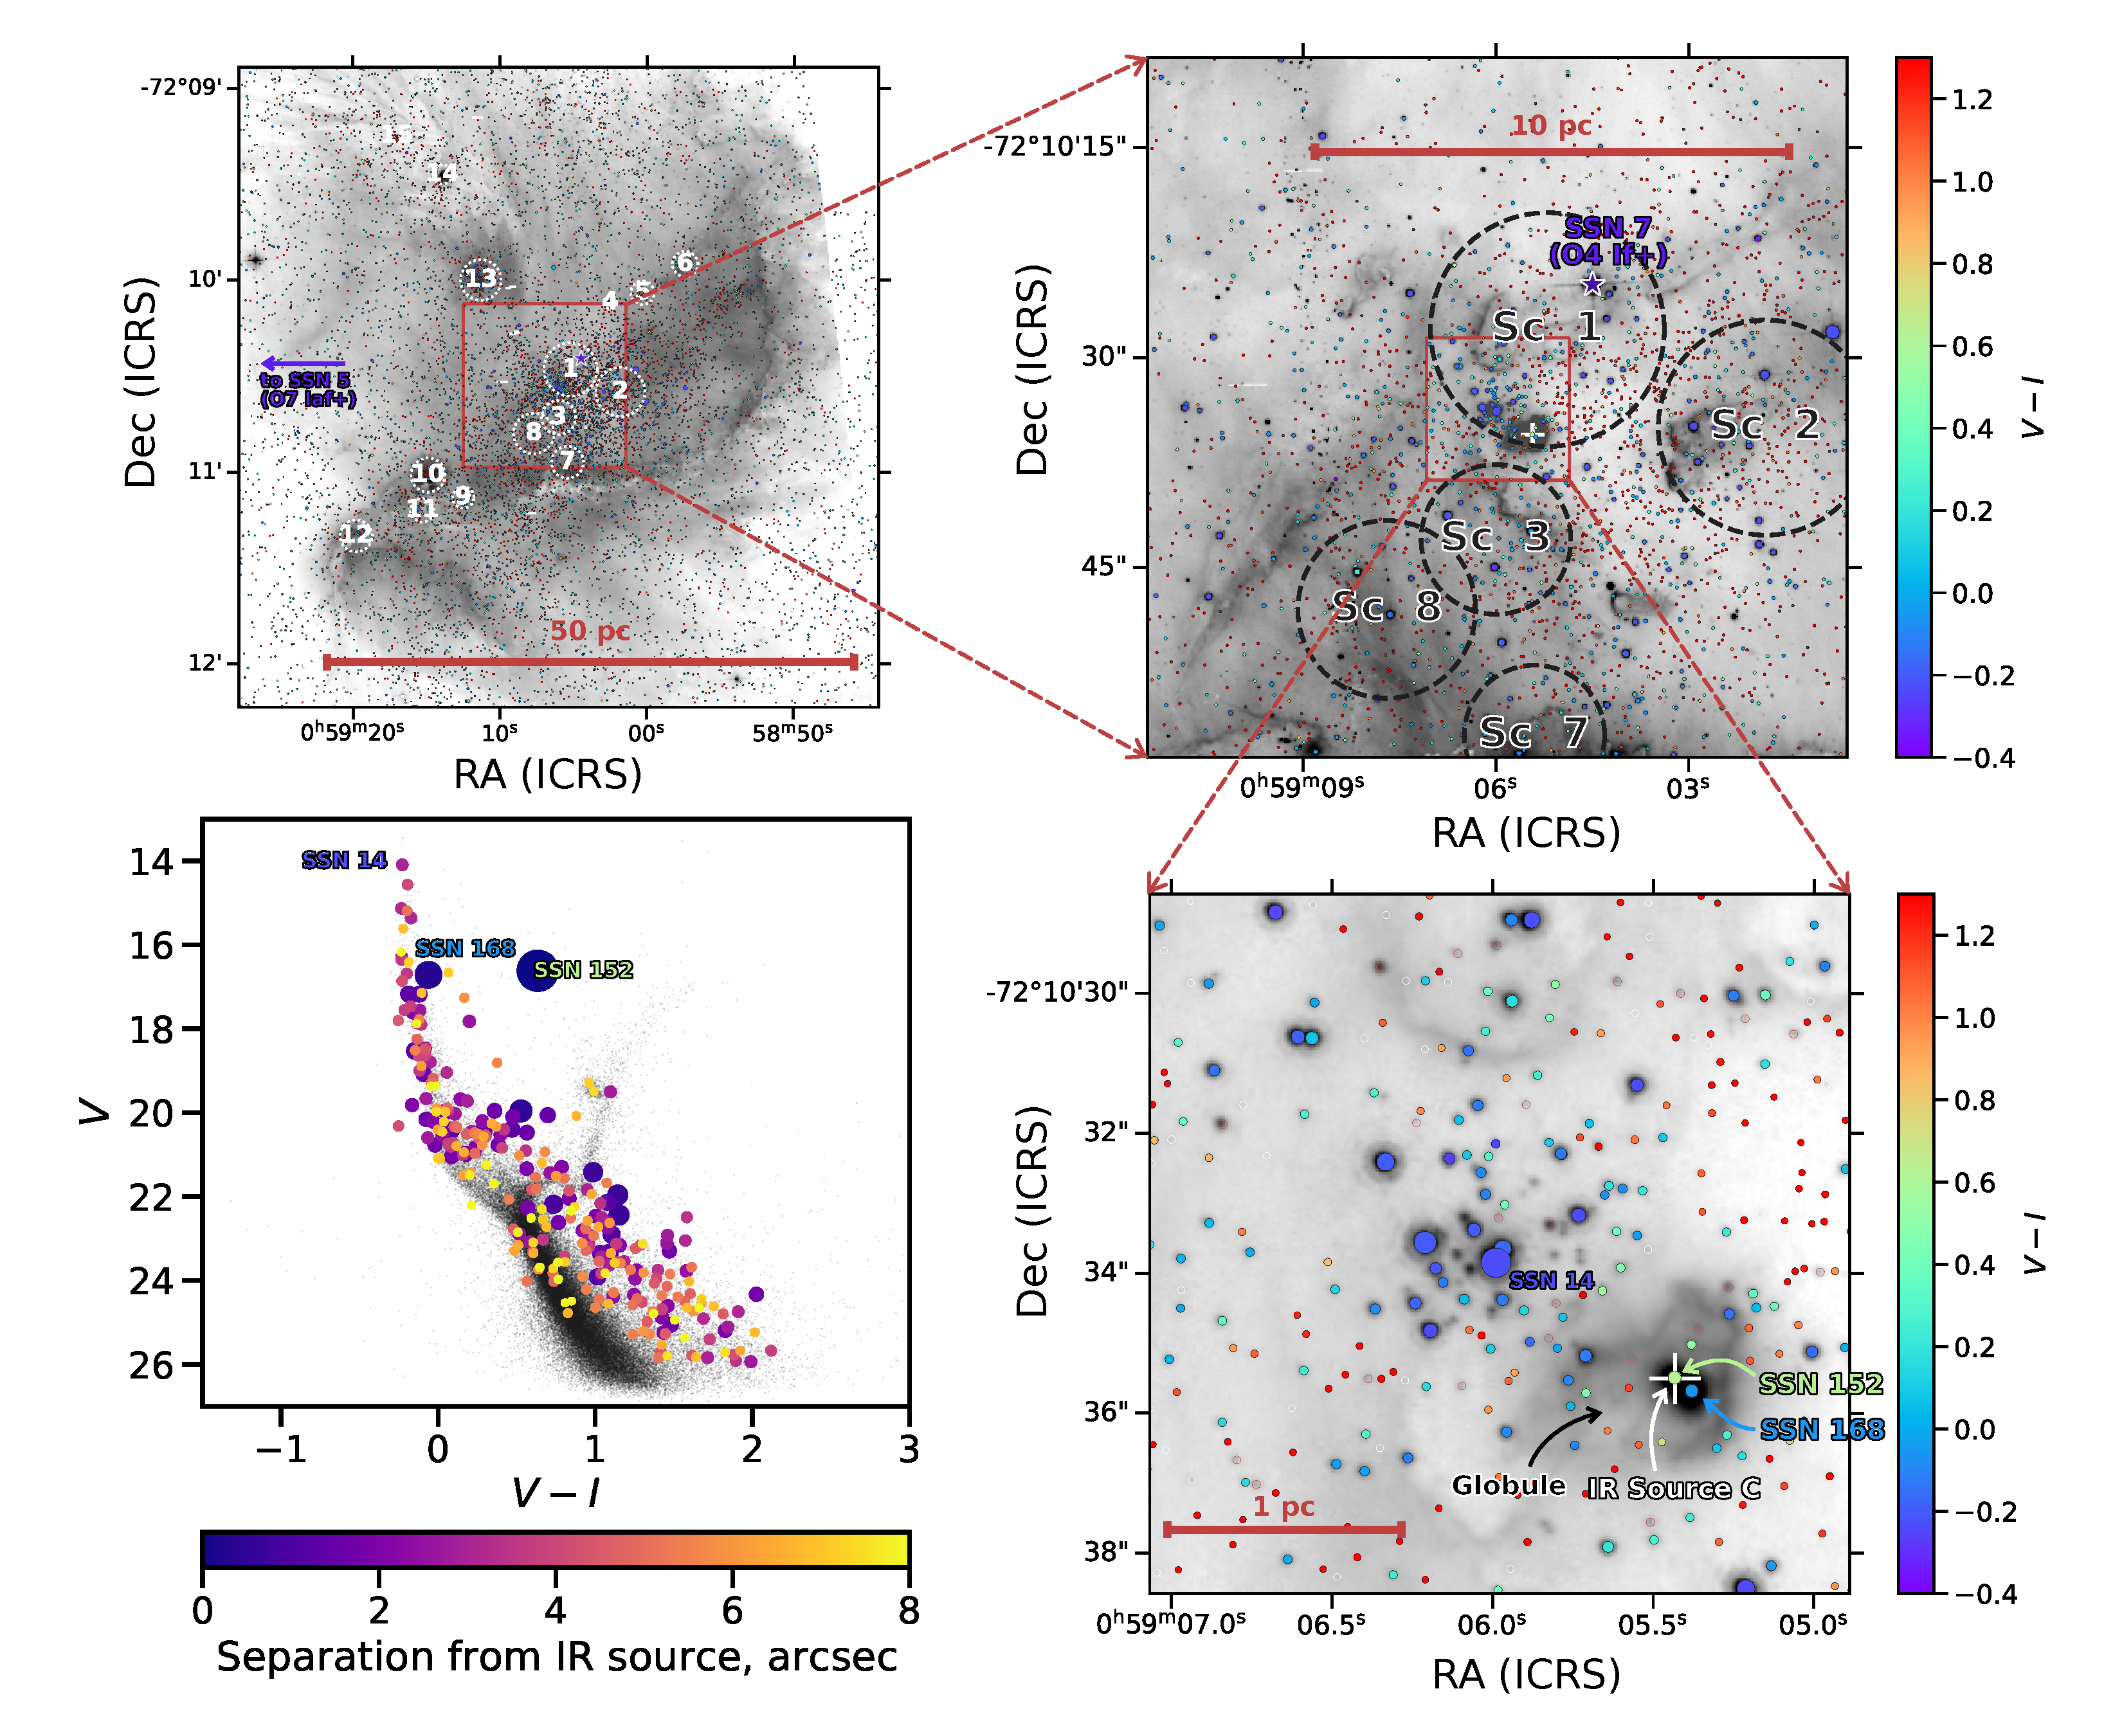
\includegraphics[width=\linewidth]{figs/ngc-346-cluster-annotated}
  \caption{Hierarchical structure of the NGC~346 star cluster.}
  \label{fig:cluster-zoom}
\end{figure*}


\section{Conclusions}
\label{sec:conclusions}

\begin{acknowledgments}
  Thank you.
\end{acknowledgments}

\facilities{VLT:Yepun (MUSE); VLA}

\bibliography{n66-refs}

\end{document}

%%% Local Variables:
%%% mode: latex
%%% TeX-master: t
%%% End:
